\documentclass[10pt,a4paper]{article}

\usepackage[utf8]{inputenc}
\usepackage[dutch]{babel}
\usepackage{amsmath}
\usepackage{amsfonts}
\usepackage{amssymb}
\usepackage{amsthm}
\usepackage{graphicx}
\usepackage{xcolor}
\usepackage{lipsum} 
\usepackage{float}
\usepackage[framemethod=default]{mdframed}
\usepackage{todonotes}

% Question command
\newtheorem{qtext}{Vraag}
\let\olddefinition\qtext
\renewcommand{\qtext}{\olddefinition\normalfont}

\setcounter{qtext}{0}
\setcounter{section}{1}

\newmdenv[skipabove=7pt,
skipbelow=7pt,
rightline=false,
leftline=false,
topline=true,
bottomline=false,
linecolor=gray,
backgroundcolor=black!8,
innerleftmargin=5pt,
innerrightmargin=5pt,
innertopmargin=0pt,
leftmargin=0cm,
rightmargin=0cm,
linewidth=2pt,
innerbottommargin=5pt]{qbox}

\newenvironment{question}{\newpage\begin{qbox}\begin{qtext}}{\end{qtext}\end{qbox}}


\newtheorem{ttext}{Definitie}

% Theorem box
\newmdenv[skipabove=7pt,
skipbelow=7pt,
backgroundcolor=black!2,
linecolor=black,
rightline=false,
leftline=true,
topline=false,
bottomline=false,
innerleftmargin=5pt,
innerrightmargin=5pt,
innertopmargin=0pt,
leftmargin=0cm,
rightmargin=0cm,
linewidth=1pt,
innerbottommargin=5pt]{tbox}

\newenvironment{theorem}{\begin{tbox}\begin{ttext}}{\end{ttext}\end{tbox}}


\newenvironment{pushcenter}{\vspace{1mm}\begin{center}}{\vspace{1mm}\end{center}}

\setlength\parindent{0pt}

\title{AUTOMATA \\ \& \\ COMPUTABILITY}
\author{\emph{Jensen Bernard}}

\begin{document}

\maketitle

\section*{Voorwoord}

Dit document bevat mogelijke examenvragen voor het vak \emph{Automaten en Berekenbaarheid}\footnote{Course G0P84a and G0P85a}, gedoceerd aan de Katholieke Universiteit Leuven. In geen enkel geval wil dit document een vervanging zijn voor de cursus. De cursustekst, \emph{Automaten en berekenbaarheid}, geschreven door \emph{Bart Demoen}, is zeer goed en het is zeker aangeraden deze grondig door te nemen voor u begint aan de volgende vraagstukken.
Ik heb dit document opgesteld tijdens het studeren van het vak, om op deze manier een overzicht te hebben van mogelijke examenvragen die we kunnen verwachten in Januari 2016. Vele vragen uit verschillende jaren komen zeer sterk overeen, daarom kan het zeker geen kwaad om deze extra aandacht te geven.
\\

Het is ook mogelijk dat er verwezen wordt naar delen uit de cursus. De meeste van deze verwijzingen zijn geschreven in December 2015. De meest recente versie was op dit moment de uitgave van 2013. Indien een nieuwere versie beschikbaar is, is het mogelijk dat de pagina's niet meer overeenstemmen. Aarzal niet om deze, zowel als mogelijke inhoudelijke fouten, aan te geven of aan te passen op Github.
\\

Ik heb vele studenten gehoord die vaak het nut niet inzien van dit vak, of dit totaal niet interessant vinden. Het is belangrijk eerst het voorwoord in de cursus eens te lezen, om een goed beeld te hebben van waar we nu eigenlijk mee bezig zijn. Indien u nog steeds van mening bent dat dit een enorm saai vak is, dan raad ik aan om ca. 2u te pauzeren om \emph{The Imitation Game}\footnote{Een film over Alan Turing, 2014} te kijken. Kom daarna terug en alles zal veel interessanter lijken dan voordien.

\newpage

\section{Talen en Automaten}

De introductie van dit hoofdstuk is op dit moment nog niet geschreven. Wanneer alle vraagstukken uit \emph{Talen en Automaten} klaar zijn, zal hier een overzicht komen van de leerstof die aan bod komt in dit hoofdstuk. Delen waar geen vragen over zijn gesteld maar wel gekend moeten zijn, zullen hier ook opgelijst worden. Zo kan dit hoofdstuk een volledig overzicht bieden van wat er over te kennen valt.
\newpage

\begin{question}
	Beschrijf in detail de transformatie van een determinitstische eindige toestandsautomaat naar een equivalente deterministische eindige toestandsautomaat met een minimaal aantal toestanden. Beschrijf de notie van equivalentie van automaten in deze context en argumenteer waarom er geen kleinere equivalente deterministische eindige toestandsautomaat bestaat. Kan een kleinere equivalente niet-deterministische eindige toestandsautomaat bestaan?
\end{question}

pagina 30 - 35
\begin{itemize}
	\item Minimale DFA uitleggen
	\item f-equivalentie uitleggen
	\item algoritme
	\item Extra: bewijs van eindigheid
	\item Isomorfe dfa's en equivalentie
	\item geen kleinere indien alles f-verschillend is
\end{itemize}

\newpage

\begin{question}
	Bespreek de twee noties ($A \leq_m B$ en $A \leq_T B$) van reduceerbaarheid, hun verband en op welke manier die noties kunnen gebruikt worden om aan te tonen dat een taal (on)beslisbaar/herkenbaar is.
\end{question}

\subsubsection*{Veel-\'e\'en reductie ($\leq_m$)}

Om over te gaan naar de definitie van de reductie van talen, kunnen we best eerst de definifie van Turing-berekenbaar erbij halen (indien we dit niet doen, kunnen we zeker zijn van deze bijvraag).

\begin{theorem}[Turing-berekenbare functie]
	Een functie $f$ heet Turing berekenbaar indien er een Turingmachine bestaat die bij input $s$ uiteindelijk stopt met $f(s)$ op de band.
\end{theorem}

\begin{theorem}[Reductie van talen]
	We zeggen dat taal $L_1$ (over $\Sigma_1$) naar taal $L_2$ (over $\Sigma_2$) kan gereduceerd worden indien er een afbeelding $f$ met signatuur $\Sigma^*_1\longrightarrow \Sigma^*_2$ bestaat zodanig dat $f(L_1) \subseteq L_2$ en $f(\overline{L_1}) \subseteq \overline{L_2}$, en zodanig dat $f$ Turing-berekenbaar is. We noteren dat door $L_1 \leq_m L_2$.
\end{theorem}

Tot hiertoe is het al duidelijk wat $L_1 \leq_m L_2$ wil zeggen. Het is nu nog belangrijk om het verband met herkenbaarheid en beslisbaarheid aan te tonen.

\begin{theorem}
	Als $L_1 \leq_m L_2$ en $L_2$ is beslisbaar, dan is $L_1$ beslisbaar.
\end{theorem}

\begin{proof}
	Het is belangrijk te weten dat de functie $f$ die elementen uit $L_1$ omzet naar element uit $L_2$ Turing-berekenbaar is. Concreet wil dit zeggen dat we de mogelijkheid hebben om een turingmachine op te stellen met als in put $s_1 \in L_1$ en als output $f(s_1) \in L_2$.\\
	Neem nu dat $L_2$ beslisbaar is, met zijn beslisser $B$. We construeren  nu een machine $C$ die elementen uit $L_1$ omzet (via $f$) naar elementen uit $L_2$, waarna we de beslisser $B$ laten beslissen. Hupsa, de combinatie van $C$ en $B$ is de beslisser van $L_1$ en ook deze taal is dus ook beslisbaar.
\end{proof}

\begin{theorem}
	Als $L_1 \leq_m L_2$ en $L_2$ is herkenbaar, dan is $L_1$ herkenbaar.
\end{theorem}

\begin{proof}
	Dit bewijs werkt hetzelfde als het voorgaande, om na te gaan dat wanneer $L_2$ beslisbaar is, dat dan ook $L_1$ beslisbaar is. Hier moeten we enkel de beslisser $B$ vervangen door een herkenner $H$.
\end{proof}

\begin{theorem}
	Als $L_1 \leq_m L_2$ en $L_1$ is niet-herkenbaar, dan is $L_2$ niet-herkenbaar.
\end{theorem}

\begin{proof}
	Stel $L_1$ is niet-herkenbaar en $L_2$ wel. We hebben zonet bewezen dat als $L_2$ herkenbaar is, ook $L_1$ herkenbaar moet zijn. Contradictie.
\end{proof}

\begin{theorem}
	Als $L_1 \leq_m L_2$ en $L_1$ is niet-beslisbaar, dan is $L_2$ niet-beslisbaar.
\end{theorem}

\begin{proof}
	Stel $L_1$ is niet-beslisbaar en $L_2$ wel. We hebben zonet bewezen dat als $L_2$ beslisbaar is, ook $L_1$ beslisbaar moet zijn. Contradictie.
\end{proof}

\subsubsection*{Orakels en hi\"erarchie van beslisbaarheid ($\leq_T$)}

De tweede notatie heeft betrekking tot orakelmachines in plaats van Turingmachines. Een orakelmachine heeft een andere structuur en werking die deze in staat stelt om, onder andere, $A_{TM}$ te beslissen. Een orakelmachine heeft bezit eigenlijk een grote map van booleans, met elke boolean behorend tot een string. Elke mogelijke string is gekoppeld aan deze $0$ of $1$ waarde. Een orakel dat een taal beslist zet alle strings die tot die taal behoren op $1$, alle andere op $0$. Door een inputstring $s$ te encoderen naar de locatie van de corresponderende booleaanse waarde, kan nagegaan worden of de string tot de taal behoort of niet. Het kan dus nooit in een oneindige lus terecht komen!
\\\\
Het nadeel is echter dat dit enkel een theoretische voorstelling is, die enkel conceptueel gebruikt kan worden. Het is onmogelijk om een bitmap met booleans te implementeren voor elke bestaande string\footnote{Want dat zijn er te veel.}.

\begin{theorem}[Turingreduceerbaar]
	Een taal $A$ is Turingreduceerbaar naar taal $B$, indien $A$ beslisbaar is relatief t.o.v. $B$, t.t.z. er bestaat een orakelachine $O^B$ die $A$ beslist. De notatie is $A \leq_T B$.
\end{theorem}

Dit is inderdaad zeer gelijkend op het eerste deel van deze vraag. In plaats van een beslisser voor $B$ te hebben, die $A$ ook beslist, gebruiken we nu een orakel. Dit orakel is dan (zoals eerder vermeld) een theoretisch hulpmiddel dat we kunnen gebruiken om onze kennis toe te passen op meerdere talen. Deze kunnen we echter in realiteit niet implementeren zoals we net beschreven hebben.

\begin{theorem}
	Indien $A \leq_T B$ en $B$ is beslisbaar, dan is $A$ beslisbaar.
\end{theorem}

\begin{proof}
	De definitie zegt ons dat $A \leq_T B$ enkel geldt indien we een orakel $O^B$ hebben dat $B$ \'en $A$ beslist. Dit is dus volledig afleidbaar van de definitie.\\
	Of anders: stel dat $B$ beslisbaar is en $A$ niet. Dan hebben we een orakel $O^B$ dat (theoretisch) $B$ beslist, maar niet $A$ (want deze is niet beslisbaar). Dit is meteen een contradictie met de definitie.
\end{proof}

\begin{theorem}
	Indien $A \leq_m B$ dan is ook $A \leq_T B$.\\
	M.a.w. $\leq_m$ is fijner dan $\leq_T$.
\end{theorem}

Dit is vanzelfsprekend indien we beseffen dat het orakel (nogmaals) een theoretische uitbreiding is op de Turingmachine. We gebruiken de Turingmachines om talen te herkennen of the beslissen. Het is mogelijk zo een machine te implementeren in een taal naar keuze. Er is echter een grens op het aantal talen dat we kunnen beslissen, aangezien een aantal in een oneindige lus kunnen komen tijdens het beslissingsproces. Dit is in de praktijk een probleem. Een theoretische oplossing daarvoor is het orakel. We kunnen deze machine wel gebruiken om theoretisch verder te redeneren. Dit will zeggen dat het orakel alle talen beslist dit een Turingmachine kan besliseen, plus de talen die een turingmachine niet kan beslissen (oneindig lus). Hierdoor is $A \leq_m B$ fijner dan $A \leq_T B$.

\newpage

\begin{question}
Bewijs dat een eindige toestandsautomaat altijd een taal herkent die door een reguliere expressie wordt beschreven. Doe dat door een eindige toestandsautomaat te transformeren naar een gegeneraliseerde niet-deterministische eindige toestandsautomaat met slechts twee toestanden.\\
Kan voor een PDA ongeveer hetzelfde gedaan worden door een gegeneraliseerde PDA op te stellen?\\
\end{question}

Voor we hier aan beginnen defini\"eren we de \emph{GNFA} als volgt:
\begin{theorem}[GNFA]
Een GNFA (gegeneraliseerde niet-deterministische eindige automaat) is een eindige toestandsmachine met de volgende wijzigingen en beperkingen:
\begin{enumerate}
\item Er is slechts 1 eindtoestand $\neq$ starttoestand
\item Er is juist 1 boog van de starttoestand naar elke andere toestand en er komen geen pijlen aan (buiten de startpijl)
\item Er is juist 1 boog van elke toestand naar de eindtoestand, maar er vertrekken geen pijlen vanuit de eindtoestand
\item Tussen elke andere 2 toestanden is er juist 1 boog in beide richtingen
\item Er is juist 1 boog van elke andere toestand naar zichzelf
\item De bogen hebben als label een reguliere expressie
\end{enumerate}
\end{theorem}
In wat volgt bewijzen we dat een eindige toestandsautomaat altijd een taal herkent die door een reguliere expressie wordt beschreven. We volgen volgend stappenplan:
$$ \text{NFA} \rightarrow \text{GNFA} \rightarrow \text{GNFA met 2 toestanden} \rightarrow \text{reguliere expressie} $$
In de opgave spreken ze van een "eindige toestandsautomaat", we gaan er hier echter vanuit dat we starten vanaf een NFA. Dit mag vermits elke DFA omgezet kan worden naar een NFA.

\begin{proof}
\subsubsection*{(a) NFA $\rightarrow$ GNFA}
We kunnen onze NFA omzetten naar een GNFA als volgt:
\begin{enumerate}
\item Maak een nieuwe starttoestand en een nieuwe (unieke) eindtoestand
\item Teken $\epsilon$-bogen van de nieuwe begintoestand naar de oude begintoestand en van elke oude eindtoestand naar de nieuwe eindtoestand.
\item Teken ontbrekende bogen met een $\phi$.
\item Als er tussen twee toestanden twee of meer parallele gerichte bogen zijn, neem die dan samen met als label de unie van de labels van de parallelle bogen.
\end{enumerate}
Nu we een GNFA geconstrueerd hebben moeten we deze reduceren naar een GNFA met 2 toestanden.

\subsubsection*{(b) Reduceren van de GNFA}
Dit doen we door herhaaldelijk een willekeurige toestand X verschillend van de start- of eindtoestand te kiezen en deze knoop de verwijderen als volgt:
\begin{enumerate}
\item Kies toestanden A en B zodat er bogen zijn van: \todo{Figuur?}
\begin{itemize}
\item A naar B met label $E_4$
\item A naar X met label $E_1$
\item X naar zichzelf met label $E_2$
\item X naar B met label $E_3$
\end{itemize}
\item Vervang het label op de boog van A naar B door $E_4 | E_1 E_2^* E_3$.
\item Doe dit voor alle koppels A en B
\item Verwijder de knoop X met alle bogen die erin toekomen of vertrekken.
\end{enumerate}
Indien er geen toestanden meer zijn, ga naar stap (c).

\subsubsection*{(c) Bepaal RE}
De GNFA heeft nu exact 2 toestanden (een start- en eindtoestand) met daartussen 1 boog. Deze boog heeft nu een reguliere expressie als label. Dit is de reguliere expressie die dezelfde taal bepaald als de oorspronkelijke NFA.
\end{proof}
\todo{bijvraag?}


\newpage

\begin{question}
	Geef een precieze formulering van het pompend lemma voor reguliere talen en een bewijs ervan. Geef voorbeelden waarbij je laat zien hoe je dat lemma gebruikt om te bewijzen dat een gegeven taal regulier is en om te bewijzen dat een gegeven taal niet regulier is.
\end{question}

pagina 43 - 45

\newpage

\begin{question}
	
\end{question}

\section{Talen en Berekenbaarheid}

\subsection{Inleiding}

\vspace{3mm}
In hoofdstuk 3, Talen en Berekenbaarheid, zal er dieper worden ingegaan op Turingmachines en de werking ervan. Na het instuderen van dit hoofdstuk is het best om onderstaande vragen op te lossen. Het zijn niet zo veel vragen, maar ze bevatten steeds een redelijk groot deel van de leerstof (vaak ook verschillende stukken gecombineerd). De vragen die volgen zijn alle vragen die al eens gesteld zijn. Deze komen echter elk jaar terug. Concreet wil dit zeggen dat als al deze vragen gekend zijn een goed resultaat verwacht kan worden.
\\\\
Dit wil echter niet zeggen dat het onmogelijk is om een andere vraag te krijgen. In de volgende sectie staat een kleine opsomming van delen uit het hoofdstuk die (tot nu toe) niet aan bod gekomen zijn tijdens de examens\footnote{Het gaat hier echter enkel over het mondeling examen, ze kunnen wel voorkomen op de tussentijds testen.}. Er bestaat echter een kleine kans dat hij zijn vragen veranderd, wat wil zeggen dat ook deze delen gekend moeten zijn. In het algemeen zijn de vragen uit dit document echter goed genoeg.
\\\\
Achteraan dit document zal ook verwezen worden naar een implementatie van een Turingmachine in Haskell. Dit kan een dieper inzicht geven op hoe zo een machine werkt.
\\\\
Aarzel niet om fouten of verbeteringen te melden op Github\footnote{User: Jense5}.

\subsection{Overige secties}

De volgende secties uit hoofdstuk 3 van Automaten en Berekenbaarheid zijn tot nu toe nog nooit aan bod gekomen op het examen, maar moeten wel gekend zijn. De pagina's komen overeen met de publicatie van 19 november 2013\footnote{De meeste recente versie in 2015.}.
\begin{enumerate}
	\item Basiswerking van een Turingmachine (p.82-86)
	\item Er bestaat een niet herkenbare taal (p.87)
	\item Universele Turingmachines (p.95)
	\item Verband met reguliere talen (p.100)
	\item $Regular_{TM}$ en $EQ_{TM}$ (p.105)
	\item Aftelbaar (p.110)
	\item The Post Correspondence Problem (p.113-116)
	\item Recursieve functies (p.122-125)
	\item De bezige bever (p.126-127)
\end{enumerate}

\begin{question}
	Formuleer en bespreek de stellingen van Church-Rosser. Geef daarbij hun belang i.v.m. het baserenvan een programmeertaal op lambda-calculus. Geef de relatie met de programmeertaal Haskell. Hoeveel conversieregels ken je?
\end{question}

\lipsum[1-2]
\begin{question}
	Bespreek de twee noties ($A \leq_m B$ en $A \leq_T B$) van reduceerbaarheid, hun verband en op welke manier die noties kunnen gebruikt worden om aan te tonen dat een taal (on)beslisbaar/herkenbaar is.
\end{question}

\subsubsection*{Veel-\'e\'en reductie ($\leq_m$)}

Om over te gaan naar de definitie van de reductie van talen, kunnen we best eerst de definifie van Turing-berekenbaar erbij halen (indien we dit niet doen, kunnen we zeker zijn van deze bijvraag).

\begin{theorem}[Turing-berekenbare functie]
	Een functie $f$ heet Turing berekenbaar indien er een Turingmachine bestaat die bij input $s$ uiteindelijk stopt met $f(s)$ op de band.
\end{theorem}

\begin{theorem}[Reductie van talen]
	We zeggen dat taal $L_1$ (over $\Sigma_1$) naar taal $L_2$ (over $\Sigma_2$) kan gereduceerd worden indien er een afbeelding $f$ met signatuur $\Sigma^*_1\longrightarrow \Sigma^*_2$ bestaat zodanig dat $f(L_1) \subseteq L_2$ en $f(\overline{L_1}) \subseteq \overline{L_2}$, en zodanig dat $f$ Turing-berekenbaar is. We noteren dat door $L_1 \leq_m L_2$.
\end{theorem}

Tot hiertoe is het al duidelijk wat $L_1 \leq_m L_2$ wil zeggen. Het is nu nog belangrijk om het verband met herkenbaarheid en beslisbaarheid aan te tonen.

\begin{theorem}
	Als $L_1 \leq_m L_2$ en $L_2$ is beslisbaar, dan is $L_1$ beslisbaar.
\end{theorem}

\begin{proof}
	Het is belangrijk te weten dat de functie $f$ die elementen uit $L_1$ omzet naar element uit $L_2$ Turing-berekenbaar is. Concreet wil dit zeggen dat we de mogelijkheid hebben om een turingmachine op te stellen met als in put $s_1 \in L_1$ en als output $f(s_1) \in L_2$.\\
	Neem nu dat $L_2$ beslisbaar is, met zijn beslisser $B$. We construeren  nu een machine $C$ die elementen uit $L_1$ omzet (via $f$) naar elementen uit $L_2$, waarna we de beslisser $B$ laten beslissen. Hupsa, de combinatie van $C$ en $B$ is de beslisser van $L_1$ en ook deze taal is dus ook beslisbaar.
\end{proof}

\begin{theorem}
	Als $L_1 \leq_m L_2$ en $L_2$ is herkenbaar, dan is $L_1$ herkenbaar.
\end{theorem}

\begin{proof}
	Dit bewijs werkt hetzelfde als het voorgaande, om na te gaan dat wanneer $L_2$ beslisbaar is, dat dan ook $L_1$ beslisbaar is. Hier moeten we enkel de beslisser $B$ vervangen door een herkenner $H$.
\end{proof}

\begin{theorem}
	Als $L_1 \leq_m L_2$ en $L_1$ is niet-herkenbaar, dan is $L_2$ niet-herkenbaar.
\end{theorem}

\begin{proof}
	Stel $L_1$ is niet-herkenbaar en $L_2$ wel. We hebben zonet bewezen dat als $L_2$ herkenbaar is, ook $L_1$ herkenbaar moet zijn. Contradictie.
\end{proof}

\begin{theorem}
	Als $L_1 \leq_m L_2$ en $L_1$ is niet-beslisbaar, dan is $L_2$ niet-beslisbaar.
\end{theorem}

\begin{proof}
	Stel $L_1$ is niet-beslisbaar en $L_2$ wel. We hebben zonet bewezen dat als $L_2$ beslisbaar is, ook $L_1$ beslisbaar moet zijn. Contradictie.
\end{proof}

\subsubsection*{Orakels en hi\"erarchie van beslisbaarheid ($\leq_T$)}

De tweede notatie heeft betrekking tot orakelmachines in plaats van Turingmachines. Een orakelmachine heeft een andere structuur en werking die deze in staat stelt om, onder andere, $A_{TM}$ te beslissen. Een orakelmachine heeft bezit eigenlijk een grote map van booleans, met elke boolean behorend tot een string. Elke mogelijke string is gekoppeld aan deze $0$ of $1$ waarde. Een orakel dat een taal beslist zet alle strings die tot die taal behoren op $1$, alle andere op $0$. Door een inputstring $s$ te encoderen naar de locatie van de corresponderende booleaanse waarde, kan nagegaan worden of de string tot de taal behoort of niet. Het kan dus nooit in een oneindige lus terecht komen!
\\\\
Het nadeel is echter dat dit enkel een theoretische voorstelling is, die enkel conceptueel gebruikt kan worden. Het is onmogelijk om een bitmap met booleans te implementeren voor elke bestaande string\footnote{Want dat zijn er te veel.}.

\begin{theorem}[Turingreduceerbaar]
	Een taal $A$ is Turingreduceerbaar naar taal $B$, indien $A$ beslisbaar is relatief t.o.v. $B$, t.t.z. er bestaat een orakelachine $O^B$ die $A$ beslist. De notatie is $A \leq_T B$.
\end{theorem}

Dit is inderdaad zeer gelijkend op het eerste deel van deze vraag. In plaats van een beslisser voor $B$ te hebben, die $A$ ook beslist, gebruiken we nu een orakel. Dit orakel is dan (zoals eerder vermeld) een theoretisch hulpmiddel dat we kunnen gebruiken om onze kennis toe te passen op meerdere talen. Deze kunnen we echter in realiteit niet implementeren zoals we net beschreven hebben.

\begin{theorem}
	Indien $A \leq_T B$ en $B$ is beslisbaar, dan is $A$ beslisbaar.
\end{theorem}

\begin{proof}
	De definitie zegt ons dat $A \leq_T B$ enkel geldt indien we een orakel $O^B$ hebben dat $B$ \'en $A$ beslist. Dit is dus volledig afleidbaar van de definitie.\\
	Of anders: stel dat $B$ beslisbaar is en $A$ niet. Dan hebben we een orakel $O^B$ dat (theoretisch) $B$ beslist, maar niet $A$ (want deze is niet beslisbaar). Dit is meteen een contradictie met de definitie.
\end{proof}

\begin{theorem}
	Indien $A \leq_m B$ dan is ook $A \leq_T B$.\\
	M.a.w. $\leq_m$ is fijner dan $\leq_T$.
\end{theorem}

Dit is vanzelfsprekend indien we beseffen dat het orakel (nogmaals) een theoretische uitbreiding is op de Turingmachine. We gebruiken de Turingmachines om talen te herkennen of the beslissen. Het is mogelijk zo een machine te implementeren in een taal naar keuze. Er is echter een grens op het aantal talen dat we kunnen beslissen, aangezien een aantal in een oneindige lus kunnen komen tijdens het beslissingsproces. Dit is in de praktijk een probleem. Een theoretische oplossing daarvoor is het orakel. We kunnen deze machine wel gebruiken om theoretisch verder te redeneren. Dit will zeggen dat het orakel alle talen beslist dit een Turingmachine kan besliseen, plus de talen die een turingmachine niet kan beslissen (oneindig lus). Hierdoor is $A \leq_m B$ fijner dan $A \leq_T B$.
\begin{question}
Bewijs dat een eindige toestandsautomaat altijd een taal herkent die door een reguliere expressie wordt beschreven. Doe dat door een eindige toestandsautomaat te transformeren naar een gegeneraliseerde niet-deterministische eindige toestandsautomaat met slechts twee toestanden.\\
Kan voor een PDA ongeveer hetzelfde gedaan worden door een gegeneraliseerde PDA op te stellen?\\
\end{question}

Voor we hier aan beginnen defini\"eren we de \emph{GNFA} als volgt:
\begin{theorem}[GNFA]
Een GNFA (gegeneraliseerde niet-deterministische eindige automaat) is een eindige toestandsmachine met de volgende wijzigingen en beperkingen:
\begin{enumerate}
\item Er is slechts 1 eindtoestand $\neq$ starttoestand
\item Er is juist 1 boog van de starttoestand naar elke andere toestand en er komen geen pijlen aan (buiten de startpijl)
\item Er is juist 1 boog van elke toestand naar de eindtoestand, maar er vertrekken geen pijlen vanuit de eindtoestand
\item Tussen elke andere 2 toestanden is er juist 1 boog in beide richtingen
\item Er is juist 1 boog van elke andere toestand naar zichzelf
\item De bogen hebben als label een reguliere expressie
\end{enumerate}
\end{theorem}
In wat volgt bewijzen we dat een eindige toestandsautomaat altijd een taal herkent die door een reguliere expressie wordt beschreven. We volgen volgend stappenplan:
$$ \text{NFA} \rightarrow \text{GNFA} \rightarrow \text{GNFA met 2 toestanden} \rightarrow \text{reguliere expressie} $$
In de opgave spreken ze van een "eindige toestandsautomaat", we gaan er hier echter vanuit dat we starten vanaf een NFA. Dit mag vermits elke DFA omgezet kan worden naar een NFA.

\begin{proof}
\subsubsection*{(a) NFA $\rightarrow$ GNFA}
We kunnen onze NFA omzetten naar een GNFA als volgt:
\begin{enumerate}
\item Maak een nieuwe starttoestand en een nieuwe (unieke) eindtoestand
\item Teken $\epsilon$-bogen van de nieuwe begintoestand naar de oude begintoestand en van elke oude eindtoestand naar de nieuwe eindtoestand.
\item Teken ontbrekende bogen met een $\phi$.
\item Als er tussen twee toestanden twee of meer parallele gerichte bogen zijn, neem die dan samen met als label de unie van de labels van de parallelle bogen.
\end{enumerate}
Nu we een GNFA geconstrueerd hebben moeten we deze reduceren naar een GNFA met 2 toestanden.

\subsubsection*{(b) Reduceren van de GNFA}
Dit doen we door herhaaldelijk een willekeurige toestand X verschillend van de start- of eindtoestand te kiezen en deze knoop de verwijderen als volgt:
\begin{enumerate}
\item Kies toestanden A en B zodat er bogen zijn van: \todo{Figuur?}
\begin{itemize}
\item A naar B met label $E_4$
\item A naar X met label $E_1$
\item X naar zichzelf met label $E_2$
\item X naar B met label $E_3$
\end{itemize}
\item Vervang het label op de boog van A naar B door $E_4 | E_1 E_2^* E_3$.
\item Doe dit voor alle koppels A en B
\item Verwijder de knoop X met alle bogen die erin toekomen of vertrekken.
\end{enumerate}
Indien er geen toestanden meer zijn, ga naar stap (c).

\subsubsection*{(c) Bepaal RE}
De GNFA heeft nu exact 2 toestanden (een start- en eindtoestand) met daartussen 1 boog. Deze boog heeft nu een reguliere expressie als label. Dit is de reguliere expressie die dezelfde taal bepaald als de oorspronkelijke NFA.
\end{proof}
\todo{bijvraag?}

\begin{question}
Geef een precieze formulering van het pompend lemma voor reguliere talen en een bewijs ervan. Geef voorbeelden waarbij je laat zien hoe je dat lemma gebruikt om te bewijzen dat een gegeven taal regulier is en om te bewijzen dat een gegeven taal niet regulier is.
\end{question}

We beginnen met dit alles intu\"itief te bekijken:\\
Stel je hebt een reguliere taal met oneindig veel strings. Er bestaat een DFA voor L met $N = \#Q$ toestanden. Neem nu een string in L die langer is dan N en begin de toch van starttoestand naar eindtoestand. Vermits er maar N toestanden zijn en je string meer dan N lang is en je bij elke overgang juist 1 symbool achterlaat, moet je op je weg naar de eindtoestand minstens 1 toestand S 2 of meer keer tegenkomen. Je hebt dus ergens een kring gemaakt. In deze string werd een substring van de oorspronkelijke string gebruikt.\\
We defini\"eren nu het pompend lemma voor reguliere talen.

\begin{theorem}[Pompend lemma voor reguliere talen]
Voor een reguliere taal L bestaat een pomplengte $d$, zodanig dat als $s \in L$ en $|s| \geq d$, dan bestaat er een verdeling van $s$ in stukken x,y en z zodanig dat s = xyz en:
\begin{enumerate}
\item $\forall i \geq 0 : xy^iz \in L$
\item $|y| > 0$
\item $|xy| \leq d$
\end{enumerate}
\end{theorem}
\todo{Eigenlijk geen def maar stelling}

In wat volgt bewijzen we deze stelling:

\begin{proof}
Neem een DFA die L bepaalt. Neem d = $\#Q+1$.\\
Neem een willekeurige string $s = a_1a_2 \hdots a_n$ met $n \geq d$. \\
Beschouw de accepterende sequentie van toestanden ($q_s = q_1,q_2,\hdots,q_f)$ voor $s$; die heeft lengte strikt groter dan $d$, dus zijn er bij de eerste $d$ zeker twee toestanden gelijk (omdat er maar $d-1$ toestanden zijn).\\
Stel dat $q_i$ en $q_j$ gelijk zijn met $i<j \leq d$ dan nemen we $x=a_1a_2\hdots a_i$ en $y=a_{i+1} \hdots a_j$ en $z$ de rest van de string. Alles volgt nu direct.
\end{proof}

Met het pompend lemma kan je \emph{niet} bewijzen dat een taal regulier is. De stelling zegt immers niet dat als het pomping lemma geldt de taal sowieso regulier is. Er kunnen nog andere condities van een reguliere taal niet voldaan zijn.
Je kan echter wel aantonen dat een taal niet-regulier is door een contradictie te bewijzen met de stelling hierboven.\\
Een soortgelijk bewijs heeft steeds de volgende structuur:
\begin{itemize}
\item Kies een willekeurig getal als pomplengte d
\item bestaat er een string langer dan d
\item waarvoor \textbf{elke} opdeling pompen verhinderd
\end{itemize}

Algemeen voorbeeld:
\begin{proof}
Stel dat er voor $L= \{a^nb^n | n \in \mathbb{N}\}$ een pomplengte $d$ bestaat. Beschouw dan de string $s=a^db^d$. Neem een willekeurige opdeling can $s=xyz$ met $|y| > 0$ dan zijn er 3 mogelijkheden:
\begin{enumerate}
\item y bevat alleen a's: dan bevat xyyz meer a's dan b's en zit deze string dus niet in $L$
\item y is van de vorm $a^ib^j$ met $i \neq 0, j \neq 0$: dan bevat xyyz niet alle a's voor de b's, en zit de string dus niet in L
\item y bevat alleen b's: dan bevat xz meer a's dan b's en zit de string dus niet in L
L kan dus niet regulier zijn.
\end{enumerate}
\end{proof}

\begin{question}
	Leg de stelling van Rice uit, en geef het bewijs. Geef minstens \'e\'en eigenschap van Turingmachines die niet voldoet aan de voorwaarde voor de stelling van Rice en toon aan dat die eigenschap geen aanleiding geeft tot een niet-beslisbare taal. Karakteriseer volledig alle eigenschappen van Turingmachines die aan de stelling van Rice voldoen m.b.v. $IsIn_{TM,S}$.
\end{question}

\subsubsection*{(a) De stelling van Rice}

Vooraleer we verder gaan met de stelling van Rice is het verstandig om sommige termen te verklaren. Niet-triviale en taal-invariante eigenschappen zijn een belangrijk onderdeel van de stelling. In onderstaande verklaringen duidt $Pos_P$ op de verzameling van machines die in het bezit zijn van een eigenschap $P$ en $Neg_P$ de verzameling van machines zonder eigenschap $P$.

\begin{theorem}[Niet-triviale eigenschap]
	Een eigenschap $P$ van Turingmachines heet niet-triviaal indien $Pos_p \neq \emptyset$ en ook $Neg_p \neq \emptyset$. Er bestaan dus Turingmachines die deze eigenschap $P$ bezitten, maar ook machines die deze niet bezitten.
\end{theorem}

\begin{theorem} [Taal-invariante eigenschap]
	De eigenschap $P$ heet taal-invariant indien alle machines die dezelfde taal bepalen hebben ofwel allemaal $P$, ofwel heeft geen enkele ervan $P$.
	$$L_{M_1} = L_{M_2} \Rightarrow P(M_1) = P(M_2)$$
\end{theorem}

\noindent Met deze twee definities in het achterhoofd, kunnen we overgaan naar de formele definitie van de stelling van Rice, met het bewijs als gevolg.

\begin{theorem}[Stelling van Rice]
	Voor elke niet-triviale, taal-invariante eigenschap $P$ van Turingmachines geldt dat $Pos_P$ (en ook $Neg_P$) niet beslisbaar is.
\end{theorem}

\begin{proof}
	We bewijzen dit met hehulp van een contradictie. Neem de Turingmachine $M_\emptyset$ die de lege taal beslist. Laten we er nu van uit gaan dat deze machine een bepaalde eigenschap $P$ heeft. De stelling zegt ons dat de eigenschap $P$ niet-triviaal en taal-invariant is. Uit de definitie kunnen we dan afleiden dat $Pos_P \neq \emptyset$ (en ook $Neg_P \neq \emptyset$). Aangezien deze verzameling niet leeg is, moet er een Turingmachine $X$ bestaan met deze eigenschap $P$. Laat ons zeggen dat deze Turingmachine de taal $L_X$ beslist.\\\\
	We gaan nu proberen een contradictie te bekomen door aan te nemen dat de stelling niet waar is. We nemen dus aan dat $Pos_P$ (en dus ook $Neg_P$) beslisbaar is. We gaan nu een beslisser $B$ proberen op te stellen voor $Pos_P$ die deze beslist\footnote{Later zullen we deze $B$ gebruiken om een beslisser $A$ te maken voor de taal met Turingmachines $A_{TM}$}. Om $B$ te maken, gaan we eerst een hulpmachine $H_{M,s}$ opstellen.\\\\
	Deze hulpmachine $H_{M,s}$ heeft een Turingmachine $M$ en een string $s$ in zich. Deze staan vast voor de machine en kunnen dus niet veranderen\footnote{Ze zijn als het ware gehardcoded.}. De input van deze machine is een string $x \in L_X$. Wanneer $H_{M,s}$ gestart wordt, zal deze eerst $M$ laten lopen over $s$. Indien $M$ $s$ reject, zal $H_{M,x}$ altijd rejecten. Indien $M$ $s$ accept, dan zal $H_{M,s}$ overgaan naar fase 2. Hier zal de hulpmachine $X$ over $x$ laten lopen. Indien $X$ $x$ ook accept, dan zal de hulpmachine accepten. Indien $X$ $x$ reject, dan zal ook de hulpmachine rejecten.
	\begin{figure}[H]
  	\centering
    	  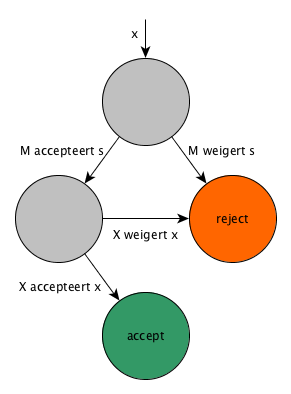
\includegraphics[width=0.3\textwidth]{./img/HMs}
  	\caption{Concept van $H_{M,s}$}
	\end{figure}
	Er zijn nu twee mogelijkheden voor $H_{M,s}$. Indien $M$ $s$ accept, dan gaat $H_{M,s}$ altijd overgaan tot het testen van $x$ in $X$. In dit geval beslist $H_{M,s}$ de volledige taal $L_X$. De andere optie is dat $M$ $s$ reject. In dat geval gaat de hulpmachine altijd rejecten en dus enkel de lege taal accepteren.\\\
	Laat nu de beslisser $B$ los op $H_{M,s}$. Dit wil zeggen dat de beslisser accept of reject voor de gegeven $M$ en $s$.\\
	Stel dat we nu een beslisser $A$ maken voor $A_{TM}$. In dat geval moeten we dus elke $M$ en $s$ in $A_{TM}$ testen. We kunnen dus zeggen dat $A$ accept indien $B$ $H_{M,s}$ accept, anders reject. We bekomen dus de volgende conclusie.
	\begin{center}
		$A$ accepts $<M,s>$\\
		$\Updownarrow$\\
		$B$ accepts $H_{M,s}$\\
		$\Updownarrow$\\
		$H_{M,s}$ heeft eigenschap $P$\\
		$\Updownarrow$\\
		$H_{M,s}$ accepts $L_X$\\
		$\Updownarrow$\\
		$M$ accepts $s$
	\end{center}
	Conclusie: $A$ is een beslisser voor $A_{TM}$, maar dit is onmogelijk aangezien $A_{TM}$ niet beslisbaar is\footnote{Zie vraag 1 van dit hoofdstuk voor het bewijs.}. Hieruit kunnen we concluderen dat alle bovenstaand equivalenties onwaar zijn en dus is  ook $Pos_P$ niet beslisbaar. Contradictie.
\end{proof}

\subsubsection*{(b) Voorbeeld}

We nemen de Turingmachine $TM$ als voorbeeld. We stellen ons de vraag over de volgende eigenschap. Zal de Turingmachine $TM$ ooit zijn leeskop naar links verschuiven? We kunnen hier een beslisser voor opstellen.
\\\\
Gegeven het tupel $<M,s>$ zal $TM$ $M$ loslaten op $s$ voor maximaal $|s|$ stappen. Als de machine geen enkele keer zijn leeskop naar links heeft bewogen, dan moet de leeskop op de eerste $\#$ staan aan de rechterkant achter $w$ op de leesband. Zoek nu de overgang $\delta$ in het state diagram van $M$ die $\#$ als input heeft. We zijn enkel ge\"intereseerd in deze, aangezien voor de andere de leeskop nooit naar links is gegaan. Indien geen enkel van deze transacties naar links gaat, accept. Indien een van hun wel naar links gaat, reject.

\subsubsection*{Algemene notatie}

De volgende notatie bepaalt de verzameling van turingmachines $M$ die een taal $L_M$ bepalen die behoord tot een gegeven verzameling van talen $S$.
$$IsIn_{TM,S}=\{<M,S>|L_M \in S\}$$
We kunnen deze notatie gebruiken om eigenschappen te karakteriseren. Een vorbeeld van een eigenschap van $E_{TM}$ die voldoet aan de voorwaarden van de stelling van Rice, is dat de bepaalde taal leeg is. We kunnen dan de volgende notatie gebruiken om de eigenschap te karakteriseren.
$$E_{TM} = IsIn_{TM,\{\phi\}}$$
\begin{question}
	Wat is een orakelmachine? Bespreek de uitspraak "de verzameling orakelmachines (over een gegeven orakel) is strikt krachtiger dan de verzameling van Turing machines". Leg hierbij ook uit wat men bedoeld met "krachtiger". Kan een verzameling orakelmachines (voor bepaald gegeven orakel) alle talen beslissen? Kan een orakelmachine ook $A_{TM}$ of $H_{TM}$ beslissen?
\end{question}

\subsubsection*{Orakelmachine}

Zoals we weten is een Turingmachine een handig hulpmiddel om te bepalen of strings tot een taal horen of niet. We kunnen de machines gebruiken om talen te herkennen, of specifieker, te beslissen. Niet alle talen kunnen echter beslist worden door zo een Turingmachine. Zo is het bijvoorbeeld onmogelijk om een Turingmachine op te stellen die de taal $A_{TM}$ beslist.
\\\\
Dit zorgt er voor dat we op zoek moeten gaan naar een betere machine die naast het beslissen van de al besliste talen, ook andere talen kan beslissen. De nieuwe machine moet dus krachtiger zijn. Het resultaat is een orakelmachine.
\\\\
Een orakelmachine is een uitbreiding op de Turingmachine, die een orakel bevat. Je kan een orakel bekijken als een black box waar de Turingmachine vragen een kan stellen. In theorie is een orakel eigenlijk een soort bitmap, of anders gezegd een rij van booleans. Stel we ordenen alle strings volgens de lexicografische orde met kortere strings eerst. Elke string op index $i$ komt nu overeen met een booleaanse waarde in de bitmap, die ook gealloceerd is op locatie $i$. Indien de string op een bepaalde locatie tot een gegeven taal $L$ behoord, dan zal de overeenkomstige booleaanse waarde op $true$ staan. Indien dit niet het geval is, blijft de waarde op $false$.
\\\\
De werking van een orakelmachine is nu heel eenvoudig. Het krijgt als input een string $s$. De machine vraagt nu aan het orakel of de string tot een taal behoort. Het orakel is in staat om de string om te vormen naar de index in de rij volgens de lexicografische volgorde en raadpleegt de overeenkomstige booleaanse waarde in de bitmap. Is die waarde $true$, dan accepteert het orakel de string $s$. Indien de waarde $false$ is, dan wordt de string $s$ geweigert. Een orakelmachine waarvan de bitmap een configuratie heeft voor een bepaalde taal $L$ te beslissen, noemen we $O^L$.

\vspace{3mm}
\begin{figure}[h!]
  \centering
      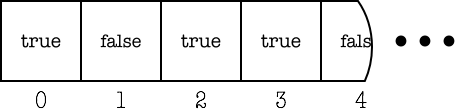
\includegraphics[width=0.5\textwidth]{./img/oracle}
  \caption{Simpele voorstelling van een orakel (bitmap).}
\end{figure}
\vspace{3mm}

Een orakel kan voor vele problemen gebruikt worden. Het halting probleem is hier echter maar \'e\'en enkel voorbeeld van. Vaak wordt een orakel gebruikt om op een abstracte manier een antwoord te krijgen op een bepaalde vraag. Deze vraag kan zelfs onoplosbaar zijn.

\subsubsection*{Krachtiger dan een Turingmachine}

Zoals zonet vermeld, is een orakelmachine krachtiger dan een Turingmachine. Dit wil zeggen dat een orakelmachine sowiso meer talen kan beslissen dan een Turingmachine. Het kan namelijk alle talen beslissen die een Turingmachine kent vermeerderd met heel wat talen die anders in een oneindige lus zullen komen. $A_{TM}$ is daar een voorbeeld van. Een orakelmachine is dus strikt krachtiger dan een Turingmachine.

\subsubsection*{Verzameling orakelmachines}

Normaal wordt een orakelmachine gegeven en kunnen we deze vraag concreet beantwoorden. Dit is nu dus onmogelijk. De redenering gaat echter van de volgende vorm zijn.
\\\\
Een orakel $O^A$ is gegeven dat een taal $A$ beslist. Volgens de definitie van Turingreduceerbaar (zie onderaan) kunnen we concluderen dat elke $B$, waarvoor geldt dat $B \leq_T A$, kan beslist worden door de orakelmachine $O^B$. Het is dus niet mogelijk om alle talen te beslissen, enkel die die Turingreduceerbaar zijn.

\begin{theorem}[Turingreduceerbaar]
	Een taal $A$ is Turingreduceerbaar naar taal $B$, indien $A$ beslisbaar is relatief t.o.v. $B$, t.t.z. er bestaat een orakelachine $O^B$ die $A$ beslist. De notatie is $A \leq_T B$.
\end{theorem}

Het is misschien wel mogelijk om een orakel te ontwerpen dat dit wel kan. In plaats van een bitmap voor alle strings, maken we een bitmap voor alle talen. Een element bevat hier geen booleaanse waarde, maar een ander orakel voor de overeenkomstige taal. Theoretisch is dit volgens mij mogelijk, maar gaat misschien iets te ver voor op het examen.

\subsubsection*{Beslisbaarheid $A_{TM}$ en $H_{TM}$}

Dit is een bijvraag en hier gaan we dus niet dieper op in. De bewijzen van de onbeslisbaarheid worden hier dus niet gegeven. Deze staan ook al in andere vragen. Volgens mij kan hier heel beknopt op geantwoord worden. $A_{TM}$ en $H_{TM}$ zijn niet beslisbaar met standaard Turingmachines. Met een orakelmachine kunnen we uiteraard een corresponderende bitmap maken voor de talen en zijn ze dus wel beslisbaar.
\begin{question}
	Geef informeel de definitie van een lineair begrensde automaat (LBA). Argumenteer dat het aanvaardingsprobleem voor LBA's ($A_{LBA}$) beslisbaar is. Geef de stappen in een bewijs dat $E_{LBA}$ (de verzameling van LBA's die de lege taal bepalen) niet beslisbaar is.
\end{question}

\subsubsection*{Lineair begrensde automaat}

\begin{theorem}[Lineair Begrensde Automaat]
	Een Lineair Begrensde Automaat is een Turingmachine die niet leest of schrijft buiten het deel van de band dat initieel invoer bevat.
\end{theorem}

De naam komt hier tot stand door de volgende equivalente definitie van een lineair begrense automaat. Deze definitie laat toe dat de $LBA$ een stuk band gebruikt dat met een constante factor $f$ groter mag zijn dan de input.

\subsubsection*{$A_{LBA}$ is beslisbaar}

Het acceptatieprobleem voor $LBA$ is gedefinieerd als de taal
\begin{center}
	$A_{LBA} = \{<M,s>|M$ \textit{is een} $LBA$ \textit{en} $s \in L_{LBA}\}$
\end{center}

\begin{proof}
	We kijken naar alle mogelijke configuraties van een $LBA$ op een string van lengte $n$. Het aantal toestanden is $q$ met het aantal elementen in het bandalfabet $b$. Het aantal mogelijke strings is dan $b^n$. De leeskop kan onder elk van de symbolen staan terwijl de machine in elk van de toestanden kan zitten. Dat geeft in het totaal maximaal $qnb^b$ configuraties.
	We kunnen nu een beslisser $B$ voor $A_{LBA}$ construeren als volgt\footnote{Bij input $<M,s>$.}:
	\begin{enumerate}
		\item Berekent $k=qnb^n$.
		\item Simuleert dan $M$ op $s$ met maximaal $k$ stappen.
		\item Indien $M$ ondertussen accepteerde, accept.
		\item Indien $M$ ondertussen verwierp, reject.
		\item Indien $M$ nog niet stopte, betekent dat dat $M$ in een lus zit en dus niet zal accepteren: reject.
	\end{enumerate}
\end{proof}

\subsubsection*{$E_{LBA}$ is niet beslisbaar}

\begin{theorem}
	$E_{LBA} = \{M|M$ \textit{is een} $LBA$ \textit{die de lege taal bepaalt} $\}$ is niet beslisbaar. 
\end{theorem}

We laten eerst zien dat voor een gegeven Turingmachine $M$ en string $s$ we een $LBA$ kunnen construeren die gegeven een eindige rij configuraties (van $M$) kan beslissen of die rij een accepterende computation history is voor $s$. Een rij configuraties kan gemakkelijk op een band geplaatst worden zoals in de figuur hieronder.
	\begin{figure}[H]
  	\centering
    	  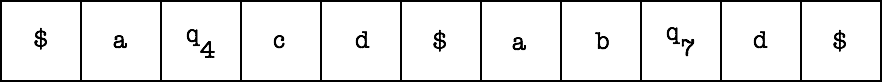
\includegraphics[width=0.8\textwidth]{./img/lba}
  	\caption{$\delta(q_4,c)=(q_7,b,R)$}
	\end{figure}
Wat moet de machine doen om na te gaan of een rij configuraties een accepterende computation history is voor $s$?
\begin{enumerate}
	\item Nakijken of twee opeenvolgende configuraties verbonden zijn door de $\delta$.
	\item Nakijken of de eerste configuratie $q_s$ bevat op de juiste plaats.
	\item NAkijken of de laatste configuratie $q_a$ bevat.
\end{enumerate}
Zonder veel in detail te treden moet het duidelijk zijn dat hiervoor slechts een constante hoeveelheid extra bandruimte nodig is en dat die beslissing dus kan  genomen worden door een $LBA$. We maken die $LBA$ zo dat hij bij een accepterende computation history accepteert en anders reject. Nu kunnen we aan het bewijs zelf beginnen.

\begin{proof}
	Stel dat we een beslisser $E$ hebben voor $E_{LBA}$. We construeren een beslisser $B$ voor $A_{TM}$ als volgt. Bij input $<M,s>$ doet $B$:
	\begin{enumerate}
		\item Construeer de $LBA$ $A_{M,s}$ die van input kan beslissen of een inputstring een accepterende computation history is voor $M$ op input $s$.
		\item Laat $E$ los op $<A_{M,s}>$: als $E$ aanvaardt, reject; anders accept.
	\end{enumerate}
	\begin{center}
		$B$ beslist $A_{TM}$ want $B$ accepteert $<M,s>$\\
		$\Updownarrow$\\
		$E$ $<A_{M,s}>$ reject\\
		$\Updownarrow$\\
		$A_{M,s}$ aanvaardt minstens \'e\'en string\\
		$\Updownarrow$\\
		Er bestaat een accepterende computation history voor $M$ op $s$
	\end{center}
	Het laatste is equivalent met zeggen dat $M$ $s$ accepteert.
	Die $B$ kan niet bestaan, dus ook $E$ niet en $E_{LBA}$ is onbeslisbaar.
\end{proof}

\newpage
\section{Herschrijfsystemen}

\subsection{Inleiding}

Het deel over herschrijfsystemen is relatief kort en makkelijk. Deze inleiding is nog niet klaar. :)

\begin{question}
	Formuleer en bespreek de stellingen van Church-Rosser. Geef daarbij hun belang i.v.m. het baserenvan een programmeertaal op lambda-calculus. Geef de relatie met de programmeertaal Haskell. Hoeveel conversieregels ken je?
\end{question}

\lipsum[1-2]
\begin{question}
	Bespreek de twee noties ($A \leq_m B$ en $A \leq_T B$) van reduceerbaarheid, hun verband en op welke manier die noties kunnen gebruikt worden om aan te tonen dat een taal (on)beslisbaar/herkenbaar is.
\end{question}

\subsubsection*{Veel-\'e\'en reductie ($\leq_m$)}

Om over te gaan naar de definitie van de reductie van talen, kunnen we best eerst de definifie van Turing-berekenbaar erbij halen (indien we dit niet doen, kunnen we zeker zijn van deze bijvraag).

\begin{theorem}[Turing-berekenbare functie]
	Een functie $f$ heet Turing berekenbaar indien er een Turingmachine bestaat die bij input $s$ uiteindelijk stopt met $f(s)$ op de band.
\end{theorem}

\begin{theorem}[Reductie van talen]
	We zeggen dat taal $L_1$ (over $\Sigma_1$) naar taal $L_2$ (over $\Sigma_2$) kan gereduceerd worden indien er een afbeelding $f$ met signatuur $\Sigma^*_1\longrightarrow \Sigma^*_2$ bestaat zodanig dat $f(L_1) \subseteq L_2$ en $f(\overline{L_1}) \subseteq \overline{L_2}$, en zodanig dat $f$ Turing-berekenbaar is. We noteren dat door $L_1 \leq_m L_2$.
\end{theorem}

Tot hiertoe is het al duidelijk wat $L_1 \leq_m L_2$ wil zeggen. Het is nu nog belangrijk om het verband met herkenbaarheid en beslisbaarheid aan te tonen.

\begin{theorem}
	Als $L_1 \leq_m L_2$ en $L_2$ is beslisbaar, dan is $L_1$ beslisbaar.
\end{theorem}

\begin{proof}
	Het is belangrijk te weten dat de functie $f$ die elementen uit $L_1$ omzet naar element uit $L_2$ Turing-berekenbaar is. Concreet wil dit zeggen dat we de mogelijkheid hebben om een turingmachine op te stellen met als in put $s_1 \in L_1$ en als output $f(s_1) \in L_2$.\\
	Neem nu dat $L_2$ beslisbaar is, met zijn beslisser $B$. We construeren  nu een machine $C$ die elementen uit $L_1$ omzet (via $f$) naar elementen uit $L_2$, waarna we de beslisser $B$ laten beslissen. Hupsa, de combinatie van $C$ en $B$ is de beslisser van $L_1$ en ook deze taal is dus ook beslisbaar.
\end{proof}

\begin{theorem}
	Als $L_1 \leq_m L_2$ en $L_2$ is herkenbaar, dan is $L_1$ herkenbaar.
\end{theorem}

\begin{proof}
	Dit bewijs werkt hetzelfde als het voorgaande, om na te gaan dat wanneer $L_2$ beslisbaar is, dat dan ook $L_1$ beslisbaar is. Hier moeten we enkel de beslisser $B$ vervangen door een herkenner $H$.
\end{proof}

\begin{theorem}
	Als $L_1 \leq_m L_2$ en $L_1$ is niet-herkenbaar, dan is $L_2$ niet-herkenbaar.
\end{theorem}

\begin{proof}
	Stel $L_1$ is niet-herkenbaar en $L_2$ wel. We hebben zonet bewezen dat als $L_2$ herkenbaar is, ook $L_1$ herkenbaar moet zijn. Contradictie.
\end{proof}

\begin{theorem}
	Als $L_1 \leq_m L_2$ en $L_1$ is niet-beslisbaar, dan is $L_2$ niet-beslisbaar.
\end{theorem}

\begin{proof}
	Stel $L_1$ is niet-beslisbaar en $L_2$ wel. We hebben zonet bewezen dat als $L_2$ beslisbaar is, ook $L_1$ beslisbaar moet zijn. Contradictie.
\end{proof}

\subsubsection*{Orakels en hi\"erarchie van beslisbaarheid ($\leq_T$)}

De tweede notatie heeft betrekking tot orakelmachines in plaats van Turingmachines. Een orakelmachine heeft een andere structuur en werking die deze in staat stelt om, onder andere, $A_{TM}$ te beslissen. Een orakelmachine heeft bezit eigenlijk een grote map van booleans, met elke boolean behorend tot een string. Elke mogelijke string is gekoppeld aan deze $0$ of $1$ waarde. Een orakel dat een taal beslist zet alle strings die tot die taal behoren op $1$, alle andere op $0$. Door een inputstring $s$ te encoderen naar de locatie van de corresponderende booleaanse waarde, kan nagegaan worden of de string tot de taal behoort of niet. Het kan dus nooit in een oneindige lus terecht komen!
\\\\
Het nadeel is echter dat dit enkel een theoretische voorstelling is, die enkel conceptueel gebruikt kan worden. Het is onmogelijk om een bitmap met booleans te implementeren voor elke bestaande string\footnote{Want dat zijn er te veel.}.

\begin{theorem}[Turingreduceerbaar]
	Een taal $A$ is Turingreduceerbaar naar taal $B$, indien $A$ beslisbaar is relatief t.o.v. $B$, t.t.z. er bestaat een orakelachine $O^B$ die $A$ beslist. De notatie is $A \leq_T B$.
\end{theorem}

Dit is inderdaad zeer gelijkend op het eerste deel van deze vraag. In plaats van een beslisser voor $B$ te hebben, die $A$ ook beslist, gebruiken we nu een orakel. Dit orakel is dan (zoals eerder vermeld) een theoretisch hulpmiddel dat we kunnen gebruiken om onze kennis toe te passen op meerdere talen. Deze kunnen we echter in realiteit niet implementeren zoals we net beschreven hebben.

\begin{theorem}
	Indien $A \leq_T B$ en $B$ is beslisbaar, dan is $A$ beslisbaar.
\end{theorem}

\begin{proof}
	De definitie zegt ons dat $A \leq_T B$ enkel geldt indien we een orakel $O^B$ hebben dat $B$ \'en $A$ beslist. Dit is dus volledig afleidbaar van de definitie.\\
	Of anders: stel dat $B$ beslisbaar is en $A$ niet. Dan hebben we een orakel $O^B$ dat (theoretisch) $B$ beslist, maar niet $A$ (want deze is niet beslisbaar). Dit is meteen een contradictie met de definitie.
\end{proof}

\begin{theorem}
	Indien $A \leq_m B$ dan is ook $A \leq_T B$.\\
	M.a.w. $\leq_m$ is fijner dan $\leq_T$.
\end{theorem}

Dit is vanzelfsprekend indien we beseffen dat het orakel (nogmaals) een theoretische uitbreiding is op de Turingmachine. We gebruiken de Turingmachines om talen te herkennen of the beslissen. Het is mogelijk zo een machine te implementeren in een taal naar keuze. Er is echter een grens op het aantal talen dat we kunnen beslissen, aangezien een aantal in een oneindige lus kunnen komen tijdens het beslissingsproces. Dit is in de praktijk een probleem. Een theoretische oplossing daarvoor is het orakel. We kunnen deze machine wel gebruiken om theoretisch verder te redeneren. Dit will zeggen dat het orakel alle talen beslist dit een Turingmachine kan besliseen, plus de talen die een turingmachine niet kan beslissen (oneindig lus). Hierdoor is $A \leq_m B$ fijner dan $A \leq_T B$.

\end{document}